\documentclass[12pt, a4paper]{article}

% Language setting
\usepackage[portuguese]{babel}

% Set page size and margins
% Replace `letterpaper' with `a4paper' for UK/EU standard size
% \usepackage[a4paper,top=2cm,bottom=2cm,left=3cm,right=3cm,marginparwidth=1.75cm]{geometry}

\usepackage[left=2cm, right=2cm, bottom=2cm, top=2cm]{geometry}

% Useful packages
\usepackage{amsmath}
\usepackage{graphicx}
\usepackage{minted}
\usepackage{verbatim}
%\usepackage[colorlinks=true, allcolors=blue]{hyperref}
%images positioning
\usepackage{array}
\usepackage[export]{adjustbox}

\title{Relatório - A2}
\author{Angel Machado \and Elainne Gutiérrez}
\date{Junho de 2025}

\begin{document}
\maketitle

\tableofcontents

\section{Introdução}
Este relatório, em \LaTeX, explica com maior abrangência as soluções dadas para as questões do trabalho de Introdução a Computação com Pandas, detalhando os tipos de dados trabalhados no processo. Depois, dedica-se a avaliar as respostas e os gráficos gerados a partir destas, contribuindo para uma análise aprofundada das dinâmicas apresentadas pela base de dados original.

\newpage
\section{Análise estatística descritiva dos dados}
A seguir apresentaremos a base de dados sobre filmes, sessões de cinema, entre outros assuntos relacionados ao cinema que utilizaremos para responder as questões e realizar uma Análise exploratória dos dados.

Temos as sete seguintes tabelas:

\begin{table}[h]
    \centering
    \begin{tabular}{l|r|r}
        Tabela       &  Numero de Linhas& Numero de colunas\\
         \hline
        distribuidora   & 72 & 3\\            
        filme	        & 515 & 6\\        
        grupo\_exibidor & 64 & 1\\           
        exibidor        & 180 & 2\\ 
        \hline
        complexo        & 683 & 4\\
        sala            & 3.231 & 3\\
        sessao          & 1.748.363 & 5\\
    \end{tabular}
    \caption{Tabelas presentes na base de dados}
    \label{tab:Tabelas das bases de dados}
\end{table}

À análise estatística dos dados de cada tabela, sera realizada da seguinte forma:

\begin{enumerate}
    \item A partir de uma Analise previa fazemos uma breve descrição sobre o conteúdo da tabela, se necessario, e definimos os tipos de dados de cada coluna de acordo com a Tabela \ref{tab:tipos_dados}
    \item exibimos as primeiras 5 linhas da tabela, onde a primeira linha que exibimos (que não faz parte da tabela) sera o tipo de dado de cada coluna
    \item Calculamos métricas simples das colunas que contenham dados discretos e datas, tais como: Media, Mediana, Quartis, Valor Máximo, Valor Mínimo, Desvio Padrão
    \item  Calculamos a Moda das coluna com dados categóricos
\end{enumerate}

cada metrica tera uma breve explicação sobre o que ela significa.

\begin{table}[h]
    \centering
    \begin{tabular}{l|r}
        Tipo & Coluna que contem\\
        \hline
        \texttt{object} & texto, rótulos\\
        \texttt{category} & valores categóricos\\
        \texttt{int64} & inteiros, dados discretos\\
        \texttt{datetime64} & datas\\
    \end{tabular}
    \caption{Tipo de dado de cada coluna de acordo com seu conteudo}
    \label{tab:tipos_dados}
\end{table}

\subsection{Distribuidora}

Contem as distribuidoras de filmes, são empresas responsáveis por levar um filme produzido ao público, cuidando da sua comercialização, divulgação e exibição em diferentes plataformas, como cinemas, televisão e plataformas de streaming.

\begin{table}[h]
    \centering
    \begin{tabular}{l|l|r}
    int64 & object & object\\
    \hline
    id    & nome   & cnpj\\
    \hline
    1& O2 PRODUÇÕES ARTÍSTICAS E CINEMATOGRÁFICAS LTDA. & 67.431.718/0001-03\\
    2& WARNER BROS. (SOUTH) INC. & 33.015.827/0001-28\\
    3& THE WALT DISNEY COMPANY (BRASIL) LTDA. & 73.042.962/0001-87\\
    \hline
    4& FREESPIRIT DISTRIBUIDORA DE FILMES LTDA. & 07.616.202/0001-01\\
    5& A2 DISTRIBUIDORA DE FILMES LTDA EPP & 18.338.912/0001-33\\
    \end{tabular}
    \caption{Primeiras linhas da tabela distribuidora}
    \label{tab:Distribuidora}
\end{table}

\newpage


\subsection{Filme}

contém os filmes que passaram nos cinemas no ano de 2023, junto com informações relevantes a cada um deles, como título, país de origem e a sua distribuidora.
\begin{table}[h]
    \centering
    \renewcommand{\arraystretch}{1.5}
    \begin{tabular}{c| m{3cm} |c|c|c|l}
    int64 & object & object & object & category & category\\
    \hline
    id & titulo\_original & titulo\_br & cpb\_roe & pais\_origem & from\_distribuidora \\
    \hline
    1&                 DURVAL DISCOS&      None&  B0200001000000&      BRASIL& 24   \\
    2&                     NOSSO LAR&      None&  B1001259400000&      BRASIL& 3   \\
    3&                       REMOÇÃO&      None&  B1301918400000&      BRASIL& 51   \\
    \hline
    4&  HOJE EU QUERO VOLTAR SOZINHO&      None&  B1402094700000&      BRASIL& 24   \\
    5&        O HOMEM DE LAGOA SANTA&      None&  B1500150500000&      BRASIL& 40  \\
    \end{tabular}
    \caption{Primeiras linhas da tabela filme}
    \label{tab:filme}
\end{table}

\begin{itemize}
    \item A moda da coluna \texttt{pais\_origem} é ESTADOS UNIDOS, são 182 filmes com esse país de origem.

    \item A moda da coluna \texttt{from\_distribuidora} é a distribuidora com id ``2" que corresponde a WARNER BROS. (SOUTH) INC. com 71 filmes que foram distribuídos por ela.
\end{itemize} 

\subsection{grupo\_exibidor}

Esta tabela apenas contém o id de cada grupo exibidor, um grupo exibidor é um conjunto de duas ou mais empresas exibidoras (cinemas) que atuam em conjunto, formando uma entidade econômica, que nesta base de dados ao total são 64.
\begin{table}[h]
    \centering
    \begin{tabular}{c}
    int64\\
    \hline
    id\\
    \hline
    5002765\\
    6000000\\
    6000002\\
    6000003\\
    6000006\\
    \end{tabular}
    \caption{Primeiras linhas da tabela grupo\_exibidor}
    \label{tab:grupo_exibidor}
\end{table}

\newpage

\subsection{exibidor}
esta tabela contém o id de cada exibidor junto com o seu respectivo grupo\_exibidor 
\begin{table}[h]
    \centering
    \begin{tabular}{c|c}
    int64 & category\\
    \hline
    id & from\_grupo\\
    \hline
    260&    6000049\\
   437&    6000013\\
   592&    6000030\\
   749&    6000058\\
  1660&    6000046\\
    \end{tabular}
    \caption{primeiras linhas da tabela exibidor}
    \label{tab:exibidor}
\end{table}

A moda da coluna \texttt{from\_grupo} é o id 6000000, com 16 exibidores, isso quer dizer que esse grupo contém 16 exibidores distintos pertencentes a um mesmo grupo empresarial responsável pela operação de salas de cinema.

\subsection{complexo}
Contém os complexos de salas de cinema (pense em um complexo como um prédio com várias salas de cinema), com a cidade e estado a que pertencem e o exibidor dono desse complexo.

\begin{table}[h]
    \centering
    \begin{tabular}{c|c|c|c}
    int64 & category & category & category\\
    \hline
         id&       municipio&  UF& from\_exibidor\\
         \hline
  438&  BELO HORIZONTE&  MG&           437\\
  895&       SÃO PAULO&  SP&          1843\\
  896&     SANTO ANDRÉ&  SP&          1843\\
  897&       SÃO PAULO&  SP&          1843\\
  898&       SÃO PAULO&  SP&          1843\\
    \end{tabular}
    \caption{Primeiras linhas da tabela complexo}
    \label{tab:complexo}
\end{table}

A moda da coluna \texttt{município} é São Paulo, com 65 complexos de cinema na cidade. Isso quer dizer, em princípio, que São Paulo em 2023 foi a cidade com mais salas de cinema do Brasil.

A moda da coluna \texttt{UF} é o estado de São Paulo (SP), com 198 complexos no estado. Interpretando da mesma forma que a moda anterior, isso quer dizer que o estado de São Paulo foi o estado com mais salas de cinema em comparação a outros estados do Brasil.

A moda da coluna \texttt{from\_exibidor} é o exibidor de id ``1843" com 85 complexos de cinema pertencentes a esse exibidor. Dando uma pesquisada rápida, poderíamos suspeitar que esse exibidor é o Cinemark.

\subsection{sala}

\begin{table}[h]
    \centering
    \begin{tabular}{c|c|c}
    int64 & object & category\\
    \hline
    id&                                         nome& from\_complexo\\
    \hline
  5000056&  KINOPLEX IGUAÇU TOP SALA 01 - KINOEVOLUTION&          2387\\
  5000057&                  KINOPLEX IGUAÇU TOP SALA 02&          2387\\
  5000058&                  KINOPLEX IGUAÇU TOP SALA 03&          2387\\
  5000061&                   SALA KINOPLEX MADUREIRA 01&          2389\\
  5000062 &                  SALA KINOPLEX MADUREIRA 02&          2389\\
    \end{tabular}
    \caption{Primeiras linhas da tabela sala}
    \label{tab:Sala}
\end{table}

A moda da coluna \texttt{from\_complexo} é o complexo de id 2620 com 18 salas de cinema, pesquisando na tabela complexo vemos que ele está na Cidade Rio de Janeiro do Estado de Rio de Janeiro. Podemos tirar uma pequena conclusão de que São Paulo é a cidade com mais salas de cinema, mas Rio de Janeiro possui o complexo com mais salas de cinema.

\subsection{sessão}

A tabela sessão é a maior tabela presente na base de dados, contendo informações sobre cada sessão registradas nas salas de cinema presentes na tabela \texttt{sala} junto com o filme e a data da sessão.

\begin{table}[h]
    \centering
    \begin{tabular}{c|c|c|c|c}
    int64 & category & category & int64 & datetime64[ns]\\
    \hline
    id& filme\_id&  sala\_id&  publico& data\_exibicao\\
    \hline
   1&      253&  5004897&        8&    2023-01-01\\
   2&      253&  5001565&       15&    2023-01-01\\
   3&      253&  5001566&       14&    2023-01-01\\
   4&      253&  5003464&       23&    2023-01-01\\
   5&      253&  5001137&       37&    2023-01-01\\
    \end{tabular}
    \caption{primeiras linhas da tabela sessão}
    \label{tab:sessao}
\end{table}

A seguir algumas métricas simples das colunas, \texttt{publico} e \texttt{data\_exibicao}

\begin{table}[h]
    \centering
    \begin{tabular}{l|c|c}
     Metrica & publico&           data\_exibicao\\
    \hline
    Media&   63&                    2023-07-01\\
    Minimo&     1&                  2023-01-01\\
    1° Quartil &   11&                    2023-04-03\\
    Mediana&   30&                     2023-07-04\\
    3° Quartil&    75&                    2023-10-02\\
    Maximo&   3.501&                2023-12-31\\
    Desvio Padrão&    95,62&              None\\
    \end{tabular}
    \caption{métricas simples da tabela sessão}
    \label{tab:sessao_metricas}
\end{table}

A moda da coluna \texttt{filme\_id} é o filme com id 256 que na tabela \texttt{filme} é GATO DE BOTAS 2: O ÚLTIMO PEDIDO com 70676 sessões

A moda da coluna \texttt{sala\_id} é a sala com id 5001791 que na tabela \texttt{sala} é SALADEARTE - CINEMA DO MUSEU da cidade de SALVADOR do estado da BAHIA , com 1176 sessões no ano de 2023

A moda da coluna \texttt{data\_exibicao} é 08/07/2023 com 6552 sessões, isso quer dizer que o dia com mais sessões foi esse.

\section{Questionário comentado}
\subsection{Questão 1}
\textbf{Qual o total de bilheteria de todos os filmes, ou seja, o público que foi aos
filmes listados?}

Fazendo o uso de \texttt{sum()}, foram somados os valores de cada linha da coluna ``\texttt{publico}", pertencente à tabela ``\texttt{sessao}'':
\begin{minted}{python}
    total_bilheteria_dataframe = sessao.publico
    total_bilheteria = sum(total_bilheteria_dataframe)
\end{minted}

A função \texttt{questao\_1} retorna um dado do tipo \texttt{`int'}, \texttt{total\_bilheteria}, que representa tal soma:
\begin{minted}{python}
    return total_bilheteria
\end{minted}

\subsection{Questão 2}
\textbf{Qual o filme de maior bilheteira em 2023, por país de origem?}

Acessamos a duas tabelas da nossa base de dados (\texttt{type(database)=`str'}), a tabela ``\texttt{filme}'' e a tabela ``\texttt{sessao}'', da primeira extraímos e guardamos na variável \texttt{id\_titulo\_pais} as colunas ``\texttt{id}'', ``\texttt{titulo\_original}'' e ``\texttt{pais\_origem}'' e da segunda guardamos na variável \texttt{filme\_id\_publico}, ``\texttt{filme\_id}'' e ``\texttt{publico}''

A abordagem para esta questão foi a partir de dicionários e o módulo do Python \texttt{defaultdict};
inicialmente criamos as seguintes variáveis com ele:

\begin{minted}{python}
    filme_de_maior_bilheteria_por_pais = defaultdict(str)
    bilheteria_de_cada_filme_por_id = defaultdict(int)
    id_de_cada_filme_por_pais = defaultdict(list)
    nome_de_cada_filme_por_id = defaultdict(str)
\end{minted}

Essas variáveis seguem o padrão \texttt{A\_por\_B} onde B é a chave do valor A, isso nos ajudou a segmentar as partes que queríamos das nossas tabelas, feito da maneira a seguir:

\begin{minted}{python}
for index in id_titulo_pais.itertuples(index= False):
        filme_id = index.id
        titulo = index.titulo_original
        pais = index.pais_origem
        id_de_cada_filme_por_pais[pais].append(filme_id)
        nome_de_cada_filme_por_id[filme_id] = titulo
\end{minted}

O método \texttt{itertuples} nos permite iterar sobre cada linha da tabela \verb|id_titulo_pais| e acessar seus valores nessas linhas, assim a variável \verb|id_de_cada_filme_por_pais| receberá cada país como uma chave, e como o valor de qualquer chave é uma lista por \texttt{defaultdict} usamos os métodos \texttt{append()} para adicionar o filme no final da lista, assim teremos um dicionário com todos os países existentes na base de dados como chave e cada chave possui uma lista dos filmes pertencentes a esse país, de maneira análoga \verb| nome_de_cada_filme_por_id[filme_id]| recebe o id como chave e o nome de cada filme como valor.

De uma maneira parecida, \verb|bilheteria_de_cada_filme_por_id| terá cada id de filme como chave e sua bilheteria total como valor

\begin{minted}{python}
    for index in filme_id_publico.itertuples(index=False):
        filme_id = index.filme_id
        publico = index.publico
        bilheteria_de_cada_filme_por_id[filme_id] += publico
\end{minted}

Com nossos dicionários criados iteramos em cada país que esteja como chave no dicionário \verb|id_de_cada_filme_por_pais|, a cada iteração instanciamos as variáveis \texttt{``bilheteria''} e \texttt{``filme''} com campos vazios, depois com cada filme que tenha esse país como chave no dicionário, comparamos se a bilheteira desse filme é maior do que a variável \texttt{``bilheteria''}, se for maior a variável é atualizada para esse valor e a variável \texttt{``filme''} é atualizada para o nome desse filme, então o dicionário\\ \verb|filme_de_maior_bilheteria_por_pais| recebe o país da iteração atual como chave e a variável \texttt{`filme'} como valor, que vai conter o nome do filme com maior bilheteira nesse país, a seguir o código:

\begin{minted}{python}
    for cada_pais in id_de_cada_filme_por_pais.keys():
        bilheteria = 0
        filme = ""
        
        for cada_filme_id in id_de_cada_filme_por_pais[cada_pais]:
            if bilheteria_de_cada_filme_por_id[cada_filme_id] > bilheteria:
                bilheteria = bilheteria_de_cada_filme_por_id[cada_filme_id]
                filme = nome_de_cada_filme_por_id[cada_filme_id]

        filme_de_maior_bilheteria_por_pais[cada_pais] = filme
\end{minted}
com isso a função retorna um DataFrame (\texttt{`pandas.core.frame.DataFrame'}), proveniente da transformação de um \texttt{`collections.defaultdict'} em uma lista (\texttt{`list'}), que por sua vez em dataframe.

\subsection{Questão 3}
\textbf{Quais são as 100 cidades com maior bilheteria em 2023, ordenadas de forma decrescente de bilheteria?}

Da tabela \texttt{`sessao'} pegamos as colunas \verb|sala_id| e público, com a função \texttt{groupby()}, agrupamos objetos iguais na coluna \verb|sala_id| ou seja, linhas com mesma id serão juntadas numa só linha, mas agora temos todos os públicos de uma só id. Com todos os públicos de uma só id usamos a função \texttt{sum()}, assim todos os públicos serão adicionados em um só, teremos como resultado: \verb|sala_id|, \verb|publico_total|, reiniciamos o \texttt{index} pois a função \texttt{groupby()} coloca \verb|sala_id| automaticamente como \texttt{index} e não queremos isso, queremos que \verb|sala_id| seja também uma coluna.

\begin{minted}{python}
sala_id_publico_total = (
        sessao[["sala_id", "publico"]]
        .groupby("sala_id").sum()
        .reset_index()
        )
\end{minted}

Da tabela \texttt{`sessao'} pegamos as colunas, \texttt{id} e \texttt{complexo}, que contêm o id de cada sala e o complexo ao qual elas pertencem. Renomeamos a coluna id para \verb|sala_id| para conseguir utilizar a função \texttt{merge()} sem muita dificuldade, com a tabela anterior.
    
\begin{minted}{python}
    sala_id_compexo = (
        sala[["id","from_complexo"]]
        .rename(columns={"id":"sala_id"})
        )
\end{minted}
Da tabela \texttt{`complexo'} selecionamos as colunas \texttt{id} e \texttt{município}, então realizamos um processo análogo ao da tabela anterior.

\begin{minted}{python}
    complexo_e_cidade = (
        complexo[["id","municipio"]]
        .rename(columns={"id":"from_complexo"})
        )
\end{minted}

Usamos a função \texttt{merge()} para juntar em uma só tabela cada tabela que temos, a partir das colunas com mesmo nome, assim conseguimos uma tabela maior com a que conseguiremos usar a função \texttt{groupby()} com cada cidade, agrupando as cidades semelhantes e somando o público total de cada uma

\begin{minted}{python}
    sala_id_publico_e_complexo = (
        sala_id_publico_total.merge(
            sala_id_compexo, how="left",on="sala_id"
            )
        )
    sala_id_publico_complexo_e_cidade = (
        sala_id_publico_e_complexo.merge(
            complexo_e_cidade, how="left",on="from_complexo"
            )
        )
    cidades_bilheteria_total = (
        sala_id_publico_complexo_e_cidade[["municipio","publico"]]
        .groupby("municipio")
        .sum(numeric_only=True)
        )
\end{minted}
Então ordenamos em ordem decrescente, pegamos as primeiras 100 linhas, reiniciamos o \texttt{index} e renomeamos as colunas.

\begin{minted}{python}
    cem100_cidades_com_mais_bilheteria = (
        cidades_bilheteria_total.sort_values(
            "publico", ascending=False
            )
        .head(100)
        .reset_index()
        .rename(
            columns={"publico": "bilheteria_total","municipio":"cidade"}
            )
        )
\end{minted}

com isso a função retorna um DataFrame (\texttt{`pandas.core.frame.DataFrame'}) de 100 linhas e 2 colunas (\texttt{cidade} e \texttt{bilheteria\_total}).

\subsection{Questão 4}
\textbf{Qual o filme com maior bilheteria em cada cidade? }

Acessamos a quatro tabelas da nossa base de dados: ``\texttt{filme}'', ``\texttt{sessao}'', ``\texttt{complexo}" e ``\texttt{sala}''. 

Renomeamos as colunas selecionadas das tabelas ``\texttt{sala}'', ``\texttt{complexo}'' e ``\texttt{filme}'' para que tenham o mesmo nome entre elas e as escolhidas da tabela ``\texttt{sessao}'', a fim de poder realizar o método \texttt{merge} entre elas. A partir da tabela ``\texttt{sala}'', selecionamos as colunas ``\texttt{id}'' e ``\texttt{from\_complexo}'', renomeando-as para, respectivamente, ``\texttt{sala\_id}'' e ``\texttt{cidade\_id}'', atribuindo esse DataFrame à variável de nome composto pelo nome das colunas; ``\texttt{sala\_id\_\_cidade\_id}":
\begin{minted}{python}
    sala_id__cidade__id = (
        sala[["id", "from_complexo"]]
        .rename(columns={"id":"sala_id","from_complexo":"cidade_id"})
        )
\end{minted}
Partindo da tabela ``\texttt{complexo}", selecionamos as colunas ``\texttt{id}" e ``\texttt{municipio}", renomeando-as para, respectivamente, ``\texttt{cidade\_id}" e ``\texttt{cidade}":
\begin{minted}{python}
    cidade_id__cidade = (
        complexo[["id", "municipio"]]
        .rename(columns={"id":"cidade_id","municipio":"cidade"})
        )
\end{minted}

A partir da tabela filme, selecionamos as colunas \texttt{id} e \texttt{titulo\_original}, renomeando a primeira para \texttt{filme\_id}.

\begin{minted}{python}
    filme_id__titulo_original = (
        filme[["id", "titulo_original"]]
        .rename(columns={"id":"filme_id"})
        )
\end{minted}

Da tabela ``\texttt{sessao}'', selecionamos as colunas ``\texttt{sala\_id}'', ``\texttt{filme\_id}'' e ``\texttt{publico}''. Agrupamos por ``\texttt{sala\_id}'' e ``\texttt{filme\_id}'' semelhantes, somando o público total de cada sala para cada filme.
\begin{minted}{python}
    sala_id__filme_id__publico_total = (
        sessao[["filme_id","sala_id","publico"]]
        .groupby(["sala_id","filme_id"])
        .sum()
        .reset_index()
        )
\end{minted}

Usamos a função \texttt{merge()} para juntar cada tabela que temos em uma só, a partir das colunas com mesmo nome. Assim conseguimos uma tabela maior de 171492 linhas e 4 colunas, sendo estas \texttt{sala\_id}, \texttt{titulo\_original}, \texttt{publico} e \texttt{cidade}.
\begin{minted}{python}
    sala_id__filme_id__publico_total__titulo = (
        sala_id__filme_id__publico_total
        .merge(filme_id__titulo_original, how="left", on="filme_id")
        )
    
    sala_id__cidade_id__cidade = (
        sala_id__cidade__id
        .merge(cidade_id__cidade, how="left", on="cidade_id")
        )

    sala_id__titulo_original__publico_total__cidade = (
        sala_id__filme_id__publico_total__titulo[["sala_id",
        "titulo_original", "publico"]]
        .merge(sala_id__cidade_id__cidade[["sala_id","cidade"]], 
            how="left", on="sala_id")
        )
\end{minted}

Assim, escolhemos todas colunas, exceto \texttt{sala\_id}, ordenamos a coluna \texttt{cidade} em ordem alfabética e os valores da coluna \texttt{publico} em ordem decrescente. Com o método \texttt{drop\_duplicates}, mantivemos apenas as linhas de primeira ocorrência de cada cidade, removendo o resto.
\begin{minted}{python}
    cidade__filme__bilheteria = (
        sala_id__titulo_original__publico_total__cidade[["cidade",
        "titulo_original","publico"]]
        .sort_values(by=["cidade","publico"], ascending=[True,False])
        .drop_duplicates(subset="cidade") 
        .reset_index(drop=True)
        .rename(columns={"cidade":"CIDADE","titulo_original":"FILME",
        "publico":"BILHETERIA"})
        )
\end{minted}

com isso a função retorna um DataFrame (\texttt{`pandas.core.frame.DataFrame'}) de 345 linhas e 3 colunas (CIDADE, FILME e BILHETERIA).

\subsection{Questão 5}
\textbf{Quais as cidades com as maiores bilheterias para filmes brasileiros?}

Analogamente à questão anterior, acessamos às quatro tabelas da nossa base de dados 
\begin{minted}{python}
    sessao = carrega_tabela(database, "sessao")
    filme = carrega_tabela(database, "filme")
    complexo = carrega_tabela(database, "complexo")
    sala = carrega_tabela(database, "sala")
\end{minted}

e renomeamos as colunas selecionadas das tabelas ``\texttt{sala}'', ``\texttt{complexo}'' e ``\texttt{filme}'' para que tenham o mesmo nome entre elas e as escolhidas da tabela ``\texttt{sessao}'', a fim de poder realizar o método \texttt{merge} entre elas. No entanto, como dessa vez escolhemos também a coluna ``\texttt{pais\_origem}" de \texttt{sala\_id\_\_filme\_id\_\_publico\_total\_\_titulo}, o DataFrame resultante do \texttt{merge} estará acrescido dessa coluna:
\begin{minted}{python}
    sala_id__titulo_original__publico_total__pais_origem__cidade = (
        sala_id__filme_id__publico_total__titulo[["sala_id",
        "titulo_original", "publico","pais_origem"]]
        .merge(sala_id__cidade_id__cidade[["sala_id","cidade"]], 
        how="left", on="sala_id")
        )
\end{minted}

Agora, agrupamos por \texttt{cidade} e \texttt{pais\_origem}, somando o público total de cada cidade por país que lançou os filmes citados no database.
\begin{minted}{python}
    cidade__pais_origem__publico = (
        sala_id__titulo_original__publico_total__pais_origem__cidade[["cidade",
        "pais_origem","publico"]]
        .groupby(["cidade","pais_origem"])
        .sum("publico")
        .reset_index()
        )
\end{minted}

Da tabela criada imediatamente acima, criamos esta aqui, escolhendo apenas as linhas cujos públicos por cidade sejam referentes a filmes brasileiros e renomeamos as colunas para os nomes pedidos pela questão
\begin{minted}{python}
    cidade__bilheteria_br = (
        cidade__pais_origem__publico
        .loc[cidade__pais_origem__publico["pais_origem"] == "BRASIL"]
        [["cidade","publico"]]
        .reset_index(drop=True)
        .rename(columns={"cidade":"CIDADE","publico":"BILHETERIA_BR"})
        
        )
\end{minted}

Pelo mesmo processo, criamos uma tabela escolhendo as linhas cujos públicos por cidade sejam referentes a filmes estrangeiros
\begin{minted}{python}
    cidade__bilheteria_estrangeira = (
        cidade__pais_origem__publico
        .loc[cidade__pais_origem__publico["pais_origem"] != "BRASIL"]
        [["cidade","publico"]]
        .groupby("cidade")
        .sum("publico")
        .reset_index()
        .rename(columns={"cidade":"CIDADE","publico":"BILHETERIA_ESTRANGEIRA"})
    )
\end{minted}
Fazemos o \texttt{merge} das tabelas sobre bilheterias brasileira e estrangeira, preenchemos seus valores nulos (NaN) com zeros e convertemos os valores de bilheterias do tipo int para o long-int, que permite realizar cálculos com valores inteiros de maior tamanho.
\begin{minted}{python}
    cidade__bilheteria_br__bilheteria_estrangeira = (
        cidade__bilheteria_br.merge(cidade__bilheteria_estrangeira, 
        how="right", on="CIDADE")
    )

    cidade__bilheteria_br__bilheteria_estrangeira["BILHETERIA_BR"] = (
        cidade__bilheteria_br__bilheteria_estrangeira["BILHETERIA_BR"]
        .fillna(0)
        .astype("Int64")
    )
\end{minted}

Com isso, a função retorna um DataFrame (\texttt{`pandas.core.frame.DataFrame'}) de 342 linhas e 3 colunas com a bilheteria brasileira em ordem decrescente e com o índice reiniciado.
\begin{minted}{python}
    return cidade__bilheteria_br__bilheteria_estrangeira
    .sort_values(ascending=False, by="BILHETERIA_BR").reset_index(drop=True)
\end{minted}

\newpage

\section{Análise exploratória dos dados}

O objetivo desta análise exploratória é entender melhor as tendências e os padrões das sessões de cinema do ano de 2023. Queremos conseguir responder às seguintes perguntas:

\begin{itemize}
    \item Quais são os 10 Filmes mais assistidos e menos assistidos nos cinemas em 2023?
    \item Qual é a media de o tempo de vida de um filme nos cinemas ?
    \item como evoluiu a compra de bilheteria e a quantidade de sessões ao longo do ano ? 
    \item Qual o dia da semana em que as pessoas mais assistem filmes nos cinemas ?
\end{itemize}

para cada pergunta iremos analisar os dados e responder com base neles, criando visualizações que permitam tirar outras conclusões além das perguntas para cumprir com o objetivo desta análise  

\subsection{Quais são os 10 Filmes mais assistidos e menos assistidos nos cinemas em 2023?}

Esta pergunta inicial pode ser respondida através da tabela \texttt{filme}, primeiramente agrupamos por filme e somamos a bilheteria de cada filme, obtendo a bilheteria total, depois contamos a quantidade total de sessões de cada filme e finalmente juntamos isso tudo em uma só tabela, que quando organizada em ordem decrescente. tera como primeiras 10 linhas os filmes com maior bilheteria enquanto as ultimas 10 os filmes com menor bilheteria, o resultado é o seguinte:

\begin{table}[h]
    \centering
    \begin{tabular}{c|c|c|l}
    \hline
    Id &	Bilheteria&	Sessões&	Titulo Original\\
    \hline
    399&	10.238.598&	56.364&	BARBIE\\
    324&	6.235.953&	64.425&	THE SUPER MARIO BROS. MOVIE\\
    329&	6.132.354&	50.614&	FAST X\\
    \hline
    269&	5.631.389&	65.808&	AVATAR: THE WAY OF WATER\\
    256&	5.358.525&	70.676&	PUSS IN BOOTS: THE LAST WISH\\
    363&	4.211.764&	40.509&	GUARDIANS OF THE GALAXY VOL. 3\\
    \hline
    360&	3.987.722&	41.205&	THE LITTLE MERMAID\\
    389&	3.985.017&	49.623&	ELEMENTAL\\
    344&	3.328.797&	36.391&	SPIDER-MAN: ACROSS THE SPIDER-VERSE\\
    455&	2.839.181&	36.641&	THE NUN 2\\

    \end{tabular}
    \caption{10 filmes com maior bilheteria}
    \label{tab:maiorbilheteria}
\end{table}

\begin{table}[h]
    \centering
    \begin{tabular}{c|c|c|l}
    \hline
    Id &	Bilheteria&	Sessões&	Titulo Original\\
    \hline
	258&	1&	1&	UNE FEMME DU MONDE\\
	34 &	3&	2&	PEQUENOS GUERREIROS\\
	47 &	4&	2&	BALA SEM NOME\\
    \hline
	223&	5&	1&	THE ROUNDUP\\
	244&	5&	2&	WHITE NOISE\\
	10 &	5&	4&	MIRANTE\\
    \hline
	200&	7&	1&	DEMON SLAYER: MUGEN TRAIN\\
	33 &	8&	1&	MIÚDA E O GUARDA-CHUVA\\
	240&	8&	2&	FOURMI\\
	26& 	9&	1&	ALÉM DA LENDA - FILME\\
    \end{tabular}
    \caption{10 filmes com menor bilheteria}
    \label{tab:menorbilheteria}
\end{table}

    é interessante perceber que dos nenhum dos 10 filmes com maior bilheteria tem como país de origem o Brasil (pois nenhum título original é em português) enquanto nos 10 filmes com menor bilheteria podemos encontrar 5 filmes com Brasil como país de origem

\newpage

\subsection{Qual é a media de o tempo de vida de um filme nos cinemas ?}

Analisaremos isto a partir do público e do número de sessões de cada filme, de forma separada.

primeiro calcularemos o tempo de vida com base na bilheteria que o filme teve em todo 2023,então dado um filme, filtramos a tabela sessão apenas com as sessões que passaram esse filme, depois agrupamos por data e somamos o público, chamaremos essa tabela \texttt{bilheteria\_por\_dia}, calculamos o 1\% do máximo da coluna que contém a bilheteria total de cada dia e agora filtramos a tabela \texttt{bilheteria\_por\_dia} para manter apenas as colunas que tiverem público maior do que 1\% do máximo que calculamos, depois somamos a quantidade total de dias que restaram e essa soma é o tempo de vida do filme.

Fazendo isso com cada filme, podemos calcular a Média, Moda e Mediana, junto com sua distribuição, do tempo de vida de um filme em relação ao público.

\begin{figure}[h]
    \centering
    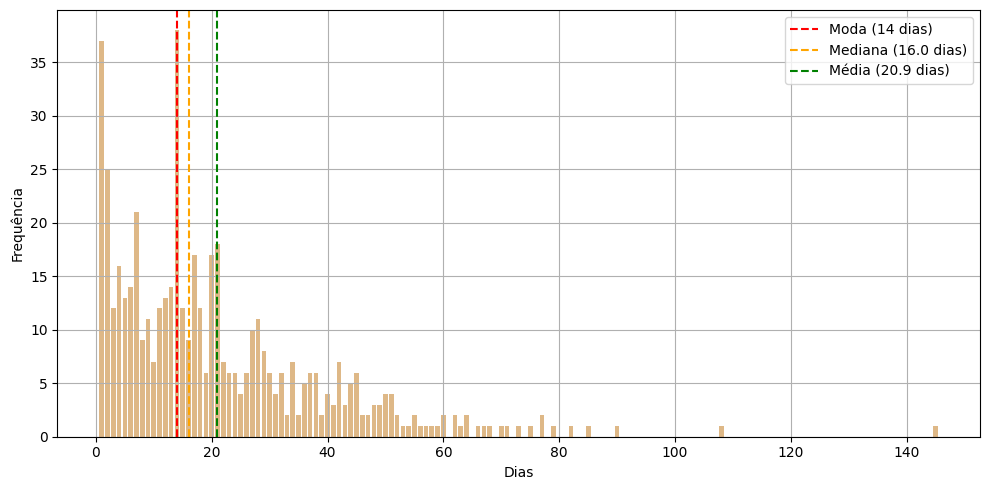
\includegraphics[width=1\textwidth]{Distribuicao_do_tempo_de_vida_bilheteria.png} % Ajuste a largura conforme necessário
    \label{fig:distribuicao_do_tempo_de_vida_bilheteria}
    \caption{Distribuição do tempo de vida em relação a bilheteria}
\end{figure}

Respondendo a pergunta inicial então podemos dizer que a média é de 21 dias aproximadamente,vendo a distribuição percebemos alguns outliers, com poucos filmes com tempos de vida superiores a 80 dias, e 37 filmes com apenas um dia de vida que puxam nossa media para baixo, então neste caso poderíamos considerar de bom grado a media de 21 dias.

Podemos então realizar o mesmo procedimento em relação ao numero de total de sessões de um filme, permanecendo apenas com os dias em que o numero de sessões foi maior ao 1\% do numero máximo de sessões que um filme já teve, assim obtendo o seguinte gráfico:

\begin{figure}[h]
    \centering
    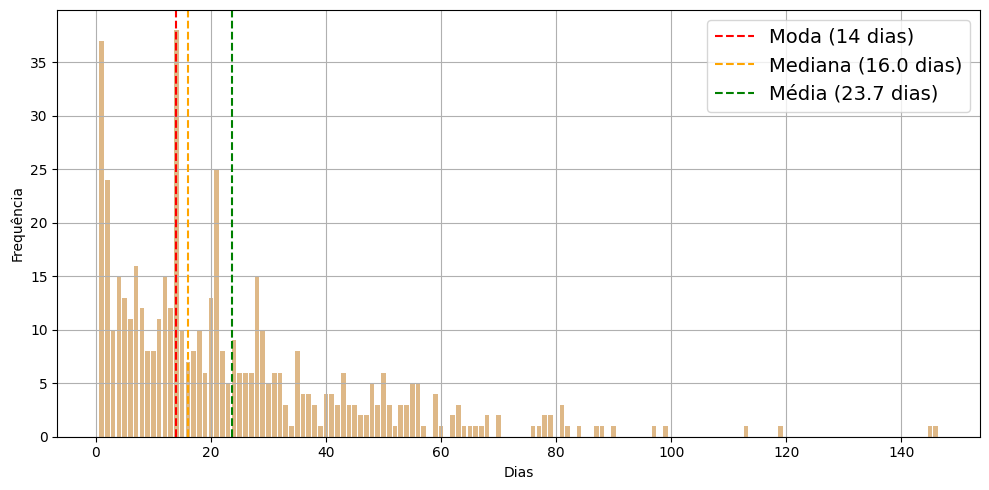
\includegraphics[width=1\textwidth]{Distribuicao_do_tempo_de_vida_sessoes.png} % Ajuste a largura conforme necessário
    \label{fig:distribuicao_do_tempo_de_vida_sessoes}
    \caption{Distribuição do tempo de vida em relação a sessões}
\end{figure}

os dois gráficos são muito parecidos, demostrando a relação entre bilheteria e o numero de sessões, é interessante perceber que a média de dias de vida em relação a de sessões é 23.7 dias e em relação a de bilheteria é 20.9 dias, com isso podemos concluir que em média um filme sai de cartela 3 dias depois da queda do seu publico.

a seguir apresentaremos dois gráficos, que mostram a evolução do publico e do numero de sessões onde se encontra refletido o tempo de vida, dos 10 filmes com maior bilheteria, a fim de curiosidade.

\begin{figure}[h]
    \centering
    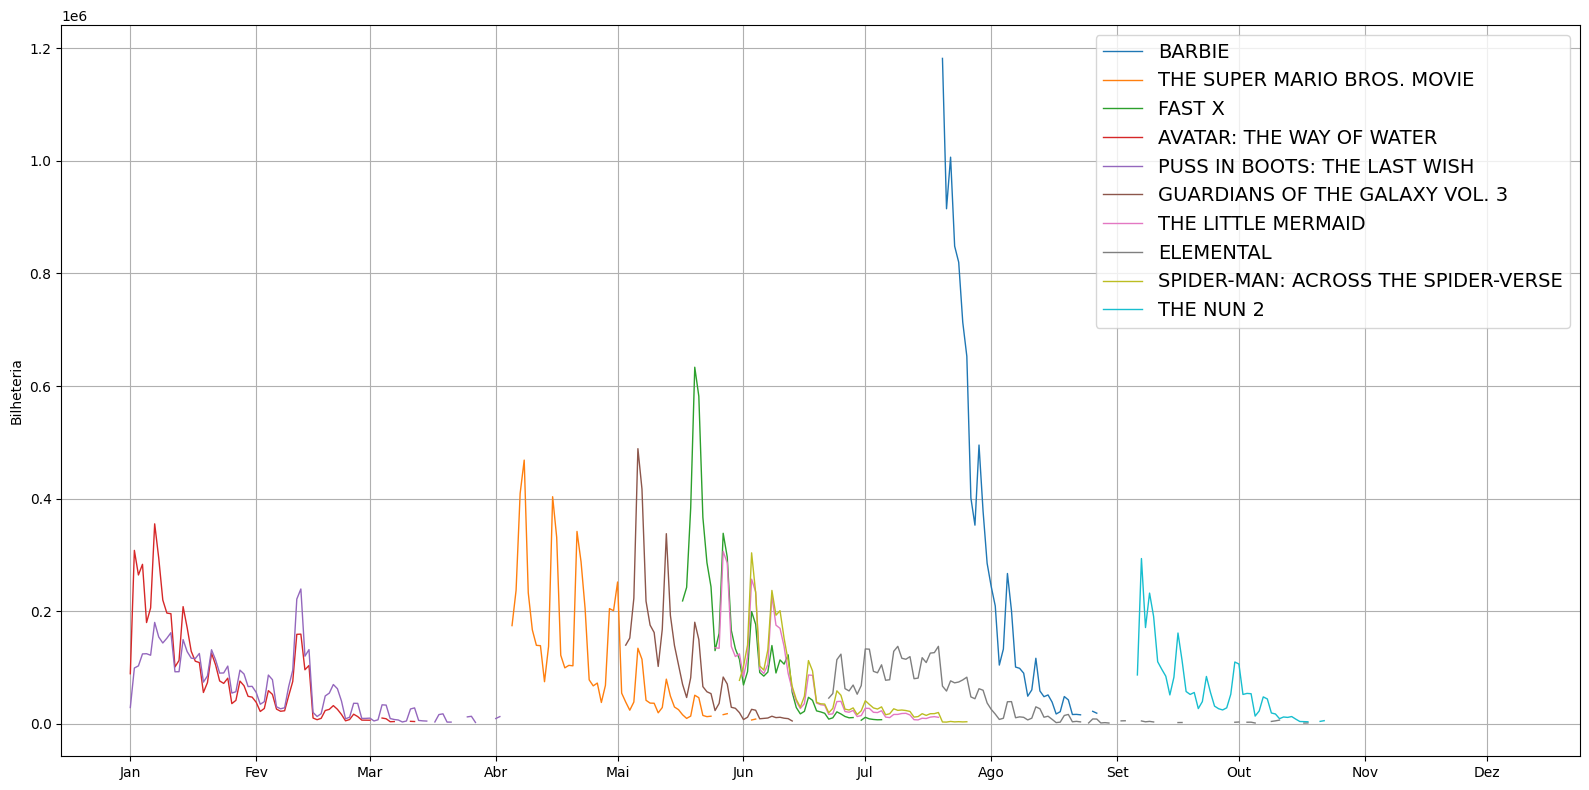
\includegraphics[width=0.9\textwidth]{tempo_de_vida_por_bilheteria.png} % Ajuste a largura conforme necessário
    \label{fig:tempo_de_vida_por_bilheteria}
    \caption{Evolução da bilheteria em relação a 1\% do seu máximo, dos 10 filmes com maior bilheteria }
\end{figure}

\begin{figure}[h]
    \centering
    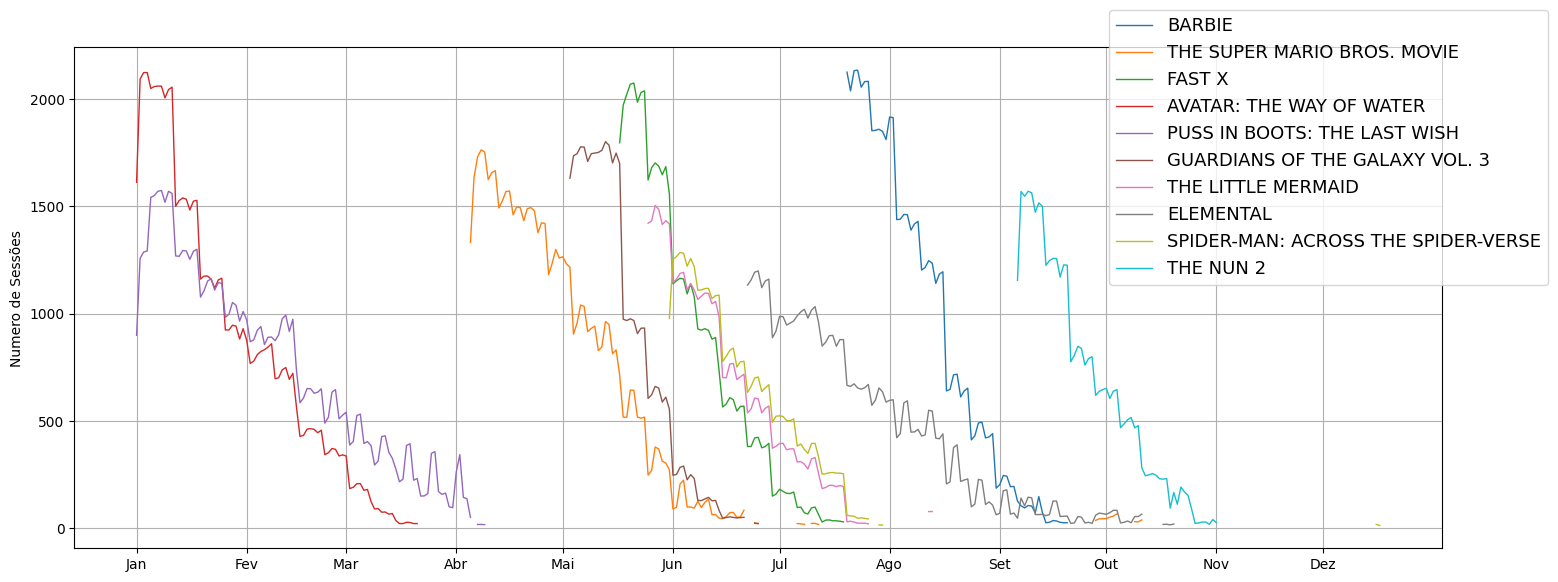
\includegraphics[width=1\textwidth]{tempo_de_vida_por_sessoes.png} % Ajuste a largura conforme necessário
    \label{fig:tempo_de_vida_por_sessoes}
    \caption{Evolução das sessões em relação a 1\% do seu máximo, dos 10 filmes com maior bilheteria }
\end{figure}

\newpage

\subsection{como evoluiu a compra de bilheteria e a quantidade de sessões ao longo do ano ?}

Para responder esta pergunta, agrupamos a tabela \texttt{sessao} por data de exibição, e somamos todos os valores da coluna \texttt{publico} assim conseguimos a serie temporal, uma maneira análoga é feita para obter a serie temporal das sessões, a seguir os graficos:

\begin{figure}[h]
    \centering
    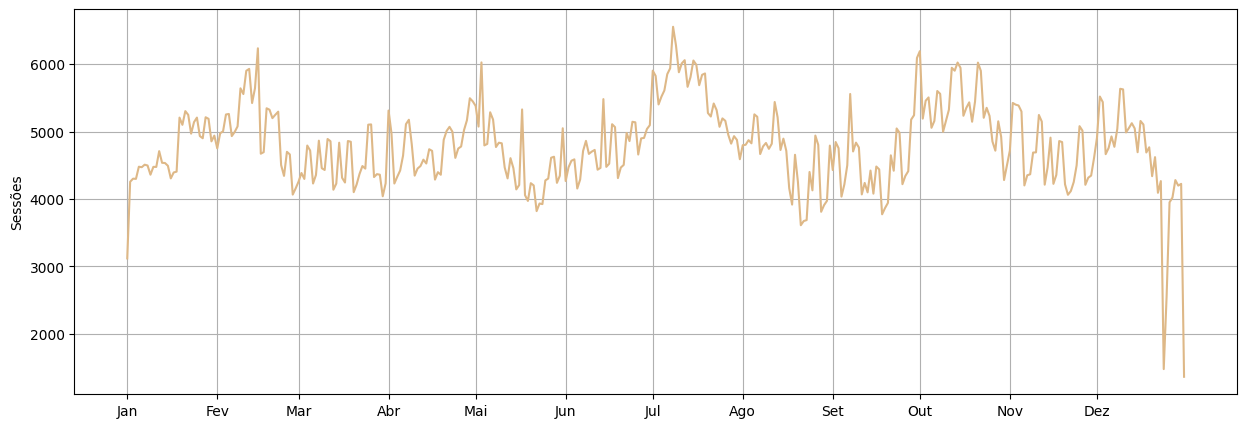
\includegraphics[width=1\textwidth]{sessoes_dia.png}% Ajuste a largura conforme necessário
    \label{fig:sessoes_por_dia}
    \caption{serie temporal por dia, das sessões do ano de 2023}
\end{figure}

\begin{figure}[h]
    \centering
    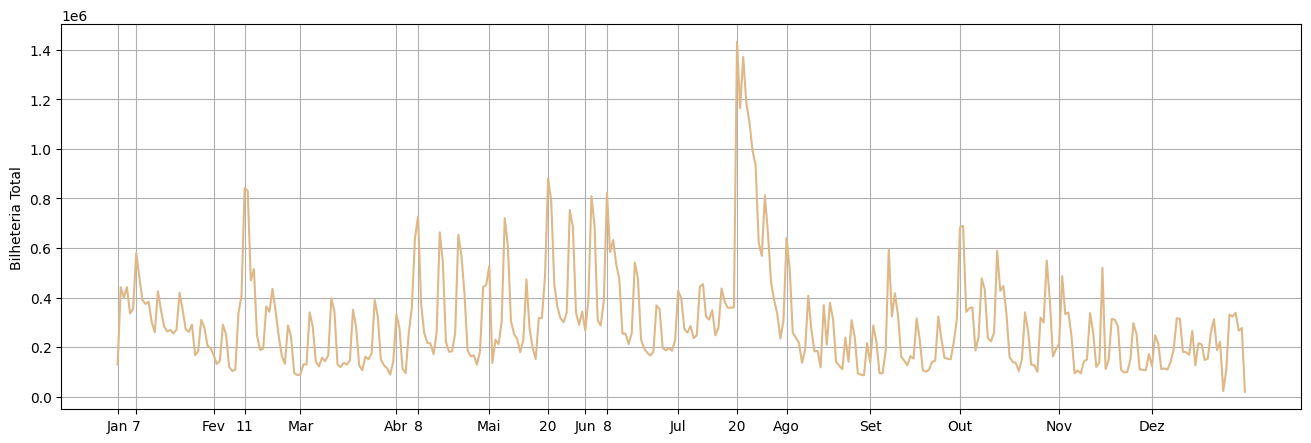
\includegraphics[width=1\textwidth]{bilheteria_dia.png}% Ajuste a largura conforme necessário
    \label{fig:sessoes_por_dia_bilheteria}
    \caption{serie temporal por dia, da bilheteria do ano de 2023}
\end{figure}

\newpage

É interessante perceber os dias de pico de cada mês da serie temporal por bilheteria. A partir de uma analise rápida podemos concluir o seguinte dos dias de pico: 

\begin{itemize}

    \item dia 10 e 11 de fevereiro que foram os dias pico, os filmes mais assistidos nesses dias foram Gato de Botas 2, Megan e Avatar que ja tinham sido estreados faz um mês mais ou menos, mas por algum motivo que é incerto, estavam tendo seu pico agora, o que sim sabemos é 11 de fevereiro foi sábado.
    \item Guardiões da Galáxia Vol. 3 estreou em 4 de maio que foi o primeiro pico de maio mas Velozes e Furiosos 10 estreou dia 18 de maio, 18 de maio foi em uma quinta feira por isso maio só teve seu segundo pico no sábado dia 20 de maio.
    \item05 de Abril tinha estreado Super Mario Brós o Filme, somente que era quarta feira, logo teve seu pico no sábado dia 8 de abril.
    \item01 de junho se estreou Spider-man: Acros the Spider-verse, mas 1 de junho foi domingo, não foi ate o sábado 8 de junho que teve seu pico.
    \item20 de julho se estreou Barbie, 20 de julho foi sábado.
\end{itemize}

\subsection{Qual o dia da semana que as pessoas mais assistem filmes nos cinemas ?}

Como vimos na sessão \textbf{4.3} todos os dias de pico foram no sábado, podemos ter a hipótese que sábado é o dia em que mais se assistem, vamos confirmar isso, agrupando a tabela \texttt{sessao} por data de exibição e separando de 7 em 7 dias, para obter cada dia da semana de segunda a domingo, depois somamos as bilheterias com dias de semana iguais.

Com isso obtemos o seguinte resultado:

\newpage

\begin{figure}[h]
    \centering
    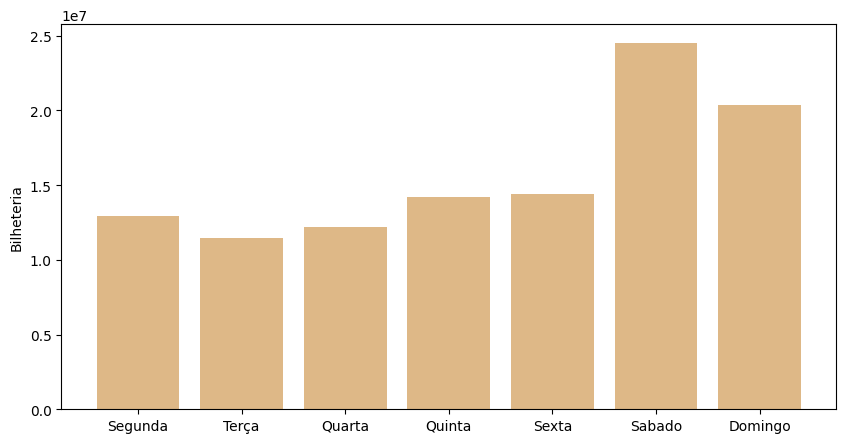
\includegraphics[width=1\textwidth]{bilheteria_dia_semana.png}% Ajuste a largura conforme necessário
    \label{fig:bilhetereria_dia_semana}
    \caption{Quantidade total de bilheteria por dia da semana }
\end{figure}

Assim confirmamos que é no sábado o dia da semana que mais se assistem filmes, junto com o domingo, já os outros dias da semana são similares.


\section{Conclusão}
Os dados analisados, possuem as bases suficientes para responder questões relevantes ao assunto, mas pode-se dizer que para se aprofundar um pouco mais nas questões precisaríamos de outros dados, estão bem organizados e prontos para uso o que facilitou nossa analise exploratória onde entendemos um pouco mais as sessões de filmes ao longo do ano, o tempo de vida médio dos filmes em cartela, as tendencias em filmes no ano de 2023, e que no final de semana é quando as pessoas mais assistem filmes.

\end{document}
